% !TEX TS-program = lualatex
%\documentclass[handout]{beamer}
\documentclass{beamer}
\input{../common/misomva}
\begin{document}
% Topic-specific title slide
\newcommand{\topictitle}{Submodularity: Applications}
\newcommand{\topicsubtitle}{Product Placement and Influence Maximization}
\newcommand{\misoclasstinytitleslide}{Partially based on material by:  Andreas Krause, \\[-1em] Branislav Kveton, Michael Kearns}

\MakeTopicSlide

\begin{frame}
\frametitle{Success story \#1 \emphcol{Product placement} - solution}

\begin{center}
% Manual layout to avoid spring layout overlap
\begin{tikzpicture}[
  marked/.style={fill=black!50},
  nd/.style={circle, draw, minimum size=8mm, inner sep=0pt},
  lbl/.style={font=\small, fill=white, inner sep=1pt}
]
\node[nd, onslide=<3-| handout:3->{marked}] (A) at (0,1.8) {A};
\node[nd] (B) at (3,1.8) {B};
\node[nd, onslide=<3-| handout:3->{marked}] (C) at (1.5,0) {C};
\node[nd, onslide=<3-| handout:3->{marked}] (D) at (0,-2) {D};
\node[nd] (E) at (3,-2) {E};
\node[nd] (F) at (1.5,-4) {F};
\only<1| handout:1>{\draw (A)--(B); \draw (A)--(C); \draw (B)--(C); \draw (C)--(D); \draw (D)--(E); \draw (D)--(F); \draw (F)--(E);}
\only<2| handout:2>{\draw[red] (A)--node[lbl,above]{0.3}(B); \draw[green] (A)--node[lbl,left]{0.5}(C); \draw[red] (B)--node[lbl,right]{0.5}(C); \draw[green] (C)--node[lbl,left]{0.5}(D); \draw[red] (D)--node[lbl,above]{0.2}(E); \draw[red] (D)--node[lbl,left]{0.2}(F); \draw[red] (F)--node[lbl,right]{0.5}(E);}
\only<3-| handout:3->{\draw[red] (A)--node[lbl,above]{0.3}(B); \draw[green] (A)--node[lbl,left]{0.5}(C); \draw[red] (B)--node[lbl,right]{0.5}(C); \draw[green] (C)--node[lbl,left]{0.5}(D); \draw[red] (D)--node[lbl,above]{0.2}(E); \draw[red] (D)--node[lbl,left]{0.2}(F); \draw[red] (F)--node[lbl,right]{0.5}(E);}
\end{tikzpicture}
 
\end{center}

\onslide<1-| handout:1->{\textbf{Key idea:} Flip coins $c$ in advance $\to$ ``live'' edges} \\
\onslide<3-| handout:3->{$F_c(V)$ = People influenced under outcome $c$ (set cover!)} \\
\onslide<4-| handout:4->{$F(V) = \sum_c P(c) F_c(V)$ is submodular as well!}\\
\onslide<5-| handout:5->{\questionbox{Computational issues?}} \moves


\par\smallskip
{\tiny \textcolor{mvaMuted}{MIIA:} \url{http://hanj.cs.illinois.edu/pdf/dmkd12_cwang.pdf/}}
\par\smallskip
{\tiny \textcolor{mvaMuted}{Tutorial: cf. Andreas Krause} \url{http://submodularity.org/}}
\par\smallskip
{\tiny \textcolor{mvaMuted}{Course: Jeff Billmes at UW}}

\end{frame}

\begin{frame}
\frametitle{Success story \#1 \emphcol{Product placement} - comparison}

\begin{center}
\textbf{influence} on the ArXiv/Physics co-authorship graph 
 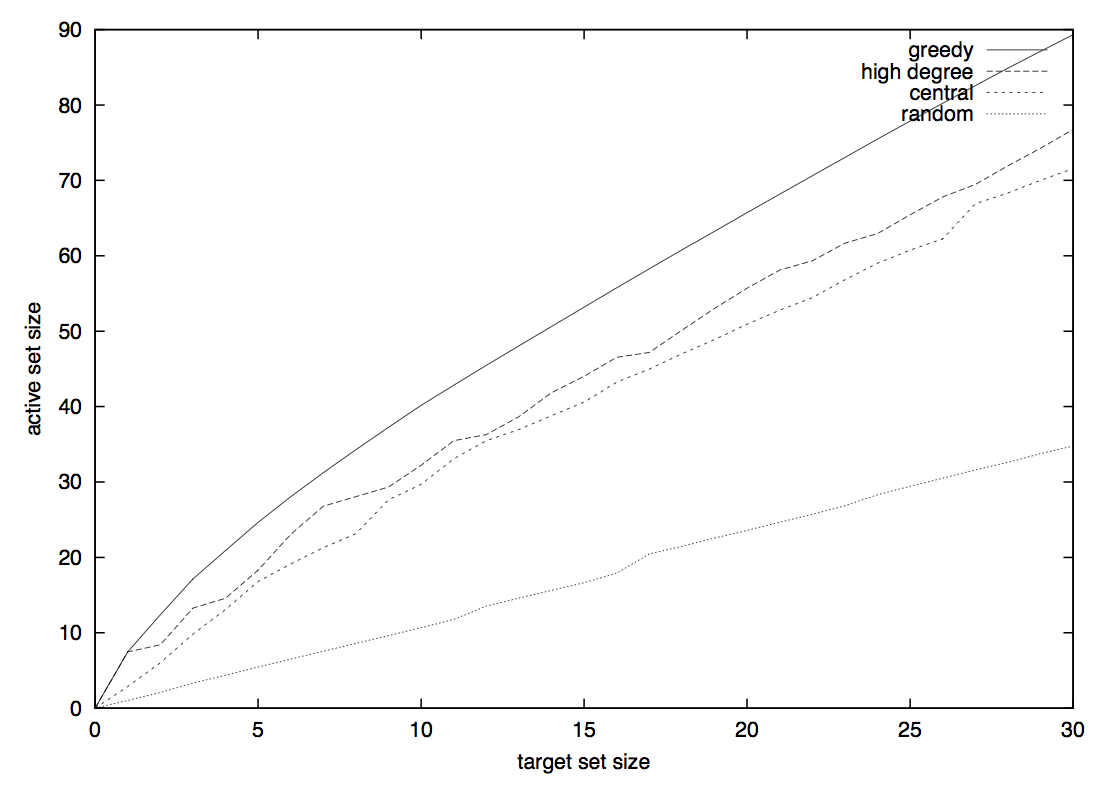
\includegraphics[width=0.7\columnwidth]{../img/kleinberg2.png}\\
{\tiny Source: Kleinberg (2000)}
 \pause
 \yellbox{greedy approximation does better than the centrality measures}
\end{center}
\end{frame}

\MakeLastSlide
\end{document}
